\chapter{Les principaux moteurs physiques}
\label{sec:solvers}

%Nous allons voir dans cette partie que plus une physique représente une part importante du contenu de l'Univers plus elle est simple et rapide a simuler.

Lors d'une simulation la grande majorité des ressources de calculs sont utilisées pour résoudre la physique.
Comme il a été abordée dans la section \ref{cosmoparam}, l'Univers est constitué de différents fluides.
Chacun étant associé à un moteur physique particulier, nous nous intéresserons dans ce chapitre à trois moteurs distincts:
\begin{itemize}
\item gravitation,
\item hydrodynamique,
\item radiatif.
\end{itemize}

%Et ce, dans un ordre décroissant d'importance, relativement a la quantité d'énergie totale.

%Plus une physique est 

Un moteur numérique consiste à estimer l'évolution de l'état d'un système, soumis a un certain nombre de règles, connaissant son état à un instant donné.
Les trois moteurs que nous allons aborder ont pour objectif de suivre des système dont l'évolution est régie par un système d'équations différentielles.
Il va être nécessaire de discrétiser ces systèmes avant de pouvoir les traiter numériquement.
L'objectif de cette partie est de présenter les différentes techniques et implémentations des moteurs physiques de EMMA.

%%%%%%%%%%%%%%%%%%%%%%%%%%%%%%%%%%%%%%%%%%%%%%%%%%%%%%%%%%%%%%%%%%%%%%%%%%%%%%%%%%%%%%%%%%%%%%%%%%%%%%%%%%%%%%%%%%%%%%%%%%%%%%%%%%%%%%%%%%%%%%%%
\section{Gravitation et matière noire}
\label{sec:solverDM}

La matière noire, dispose de propriétés de fluide non collisionelle, et se prête particulièrement bien à la représentation Lagrangienne, et donc a une simulation sous forme de particule.
Pour la simuler, on utilisera le principe des code N-corps., c'est à dire qu'on utilisera un champs de particules massive interagissante uniquement par gravitation.
Il existe différentes techniques pour suivre l'évolution d'un tel système, toutes sont basées sur le même principe.
Les particules sont placée suivant une certaine condition initiale et on cherche à connaitre la force gravitationnelle à laquelle chaque particule est soumise, dans le but de calculer son déplacement.

\subsection{Génération des conditions initiales}
\label{sec:IC}

Nous avons vu (cf \ref{sec:CMB}) que le \ac{CMB} nous donne de l'information sur l'état de la distribution de matière dans l'univers très tôt dans son histoire.
Il est possible de déterminer le spectre de puissance des fluctuations de densité de l'univers primitif à partir du \ac{CMB}.
Le principe de la génération des condition initiales est d'utiliser ce spectre de puissance pour générer des surdensité représentant statistiquement ces fluctuations.
Pour se faire on va générer une grille régulière sur laquelle on placera une particule au centre de chaque cellule, dans ce cas la densité est homogène.
On va alors perturber la position des particules de manière à respecter les fluctuations statistique observées dans le \ac{CMB}.
Pour ce faire, on va générer un bruit aléatoire Gaussien que l'on 
%Tout les générateurs de condition initiales que j'ai pu rencontrer utilise une SEED aléatoire, dans le but de générer ce bruit aléatoire.
convoluera ensuite avec le spectre de puissance que l'on cherche a reproduire.
On déplacera finalement les particules en accord en leurs appliquant les perturbations obtenues. 
Cette approximation est l’approximation de Zeldovitch (voir eg \cite{2014MNRAS.439.3630W}) et n'est valable que dans le cas des petites perturbations, tant que l'on reste dans le régime linéaire.
%L’approximation de Zeldovitch est capable de prédire analytiquement la distribution de la matière à très grandes échelles.
%Mais plus l'on cherche à étudier des petites échelles, plus on sort vite du domaine de précision acceptable.
En dehors de cette approximation, il est nécessaire d'avoir recourt aux simulations numériques.

Nous voyons ici que le spectre est limité des deux cotés.
D'un coté l'information des grandes échelles est tronquée par la taille de la boite considéré et il n'est pas possible d'avoir de l’information sur des longueurs d'onde du spectre plus grande que cette taille limite.
De l'autre coté, les petites échelles sont tronquées par la limite de résolution et le spectre est troqué au niveau de la longueur d'onde correspondant à la résolution de la grille.
Cette perte d'information sur les hautes fréquences peux être problématique dans le cas où la résolution est adaptative.
%Dans le cas de l'\ac{AMR} par exemple il peux paraître difficile d'autoriser un nombre élevé de niveau de raffinement puisque les niveaux nouvellement créer ne disposerons pas de l'information des conditions initiales.

%En pratique j'ai principalement utilisé MUSIC et GRAPHIC %TODO ref.

%méthode
%gaussian random noise
%théorie des perturbation linéaire
%lien avec le spectre de puissance
%MUSIC et GRAPHIC
%limite la résolution min et max (min en masse et max en espace)


%une simulation est limité par sa taille et sa résolution -> ceci définit la plage d'échelle que l'on peut simuler
%
%principes de bases ennoncé dans Pen (1997) and Bertschinger (2001).
%
%    discrétisation de l'espace
%    placement des particules sur la grille
%    génération d'un bruit blanc
%    convolution avec un spectre de puissance connu (celui du CMB)

%
%\subsection{Théorie des perturbation linéaire}
%
%approximation de zeldovich
%perte de linéarité a un certain moment -> nécessité des simulation numériques

\subsection{Moteur de gravité}
\label{sec:gravity}

%Je vais plus détailler le solveur de gravité que les autres puisque c'est celui sur lequel j'ai le plus travaillé.
%Le sloveur que je connais le mieux.
%Fluide non collisionnel -> particule\\

A partir des conditions initiales générées, on cherche ensuite à suivre dynamiquement l'évolution des particules.
Le but est d'obtenir la position des particules à chaque instant.
%Pour cela, il faut leurs vitesses.
%Pour cela, il faut leurs accélération.
%Pour cela, il faut la force qui leur est appliquée.
%Et dans certain cas, il faut le potentiel gravitationnel.
Ce système d'équations est appelé le système d'équation de Vlasov-Poisson :

\begin{equation}
\begin{cases}
\frac{d{x}_p}{dt} = { v}_p, \\
\frac{d{ v}_p}{dt} = -\nabla \phi , \\
\Delta \phi= 4\pi G \rho.
\end{cases}
\label{eq:Ncorps}
\end{equation}

Il existe plusieurs méthodes pour résoudre ce système.
%Historiquement la première méthode était la méthode
\paragraph{Particule-Particule (PP) : } c'est la méthode la plus directe pour calculer l'évolution d'un system N-corps. 
Elle consiste, pour chaque particule, à sommer les contributions gravitationnelles de toutes les autres particules:
\begin{equation}
\vec{F}_i=-\sum_{j\neq i} G \frac{G m_i m_j(\vec{r}_i - \vec{r}_j) }{ |\vec{r}_i - \vec{r}_j |^3}
\end{equation}
Ce type de code dispose d'une très bonne précision mais la quantité de calculs évolue en ordre $O(N^2)$, ce qui fait que ce type de code est très coûteux.

%Une évolution de cette méthode est la méthode :
\paragraph{Tree code: } évolution de la méthode PP, elle consiste à regrouper les particules les plus lointaine de la particule courante en amas aillant une interaction gravitationnelle commune \citep{1986Natur.324..446B}.
% (Barnes & Hut 1986) 
Cette approximation permet de limiter considérablement le nombre de calcul, ordre $O(n log n)$, pour les interactions lointaine qui sont de toute façons faibles 



%On peux obtenir cette force soit par calcul direct, soit par dérivation du potentiel.
%
%\begin{equation}
%\vec{F}=-\Delta \Phi
%\end{equation}


\paragraph{Particule-Mesh (PM) : } La méthode qui nous intéresse ici.
Elle consiste à ne plus calculer directement la force, mais à la dériver à partir du potentiel.
Le potentiel sera calculé sur une grille.
En projetant les particules sur une grille on obtient une grille de densité utilisée ensuite obtenir le potentiel en résolvant l'équation de Poisson.
%ENZO %code, Bryan & Norman 1998
%RAMSES

\paragraph{}
La méthode de projection des particules sur la grille n'est pas unique.
A l'ordre $0$, il est possible de se contenter d'ajouter la masse de la particule dans la cellule a laquelle elle appartient.
On utilisera en pratique une méthode d'ordre supérieur appelée \ac{CIC}:

\paragraph{CIC} : consiste à considérer une étendue spatiale aux particules et à pondérer la masse appliquée aux cellules par l'intersection de son volume et de celui de la cellule (voir Fig\,\ref{fig:CIC}).
On associe généralement une taille à la particule similaire a celle des cellule sur laquelle on la projette.
Dans le cas où l’étendue de la particule intersecte des cellules de différents niveaux on lui associera la taille de la plus grande cellule dans le but de lisser la transition entre les niveaux.
%Il existe des méthodes d'ordre supérieur avec des kernel plus complexe que le top-hat du \ac{CIC} comme par exemple des kernel en triangle ou en gaussienne.
%http://techfinder.stanford.edu/technology_detail.php?ID=30866

\begin{figure}
		\centering
        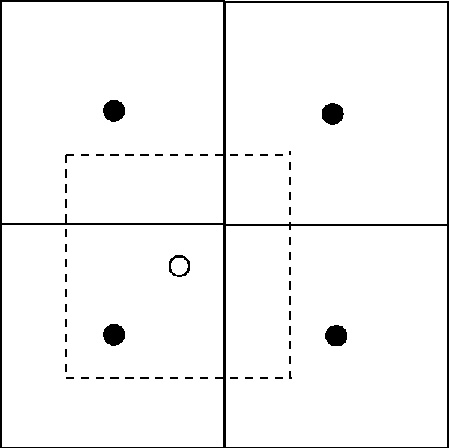
\includegraphics[width=.5\linewidth]{img/02/CIC.jpg} 
        \caption[CIC]{Représentation en 2D du Cloud In Cell. 
        La masse d'une particule est répartie dans le cellules environnantes en lui associant une étendue spatiale.
        %http://homepage.univie.ac.at/franz.vesely/cp_tut/nol2h/new/c6sm_s4lr.html
 		\label{fig:CIC}}
\end{figure}

\paragraph{}
Une fois la grille de densité générée, nous pouvons calculer le potentiel en résolvant l'équation de Poisson.

\subsubsection{L'équation de Poisson}

Connaissant la distribution de densité à un instant donné, il est possible de calculer le potentiel gravitationnel en résolvant l'équation de Poisson:

\begin{equation}
\Delta \Phi = S_{(\rho)}
\end{equation}

où :
\begin{equation}
S_{(\rho)} = 4 \pi G \rho
\end{equation}
dans le cas classique, et devient en système d'unité supercomobile (cf Sec. \ref{sec:supercomobil}):
\begin{equation}
S_{(\rho)} = 6 a \delta_{(\rho)}
\end{equation}
avec le contraste de densité: 
\begin{equation}
\delta_{(\rho)} = \rho / < \rho > - 1 
\end{equation}

En intégrant deux fois la distribution de densité on obtient le potentiel gravitationnel:

\begin{equation}
\Delta \phi = S \longrightarrow \phi = \iint \Delta \phi = \iint S_{(\rho)}
\end{equation}

Pour cela, il existe principalement deux types de méthodes. 
La première est basée sur les transformées de Fourier. 
Cette méthode, très rapide, utilise le fait que dans l'espace de Fourier, une intégrale se résume à une division par un nombre d'onde. 
Déterminer le champ de potentiel revient à : 
\begin{itemize}
\item Effectuer la transformée de Fourier de la densité
\item Diviser par $k^2$
\item Effectuer la transformée de Fourier inverse
\end{itemize}

\begin{equation}
S_{(\vec{x})} \overset{FFT}{\longrightarrow}  S_{(\vec{k})} \times \frac{1}{k^2}  \overset{RFFT}{\longrightarrow}  \phi_{(\vec{x})}
\end{equation}

De par la nature des transformées de Fourier, le champ de densité doit être périodique pour que l'implémentation de cette technique ne se révèle pas trop complexe. 
Ce qui n'est pas un problème en simulation cosmologique, où les conditions de bords sont toujours périodiques mais est plus problématique lors de la simulation de structures isolées, telles les galaxies ou les amas de galaxies. 
De plus, les \ac{FFT} nécessitent un échantillonnage régulier, ce qui implique que cette méthode est incompatible avec les méthodes \ac{AMR}. 
%Et dernièrement, le passage dans l'espace des fréquences nécessite des conditions de types plans parallèles lors parallélisation, conditions incompatible avec la gestion de grille utilisé par les code AMR dont EMMA} fait partie. \\

Le second type de méthodes est dit itératif. 
Il consiste à faire converger le potentiel à partir d'une condition initiale arbitraire. 
Ces méthodes sont plus lente que la méthode par \ac{FFT} mais permet d'utiliser tout type de conditions de bords, d'être facilement parallélisable et d'être compatible avec les méthodes basées sur des grilles adaptatives.
%Par la suite, c'est donc une méthode itérative et plus précisément une méthode \emph{Multigrille} qui à été développée.
%Le potentiel est alors dérivé pour obtenir la force ressentie dans chaque cellule. 
%Il est ensuite aisé de calculer l'accélération subie par les particules de chaque cellule, et par intégration temporelle, leurs nouvelles positions et vitesses.
Le principe de ces méthodes est d'introduire un terme temporel fictif et de rechercher un solution stationnaire à cette nouvelle équation.
Par analogie à l'équation de la chaleur par exemple, la densité correspond aux sources chaudes et le potentiel à la température, à $t=0$ les sources chaudes sont allumées et la chaleur se propage jusqu'à ce que le milieu ait atteint sa température d'équilibre. 
%Ici, c'est la gravité qui se diffuse dans le milieu.
L'équation à résoudre est donc:

\begin{equation}
\dfrac{\partial \phi}{\partial t} = \Delta \Phi -S_{(\rho)}
\end{equation}



\subsubsection{Méthode jacobi}

La méthode de Jacobi est la façon la plus simple de relaxer ce type d'équation, elle consiste à utiliser directement la forme discrète de l'équation de Poisson modifiée. 
L'équation à intégrer est:

\[ \dfrac{\phi^{t+1}_i - \phi^{t}_i}{\Delta t}  =  \Delta \phi_i^t - S_i^t \]

où, à 3 dimensions, le Laplacien s'exprime :

\[ \Delta \phi_i^t = \dfrac{\phi_{x+1,y,z}^t  + \phi_{x-1,y,z}^t + \phi_{x,y+1,z}^t  + \phi_{x,y-1,z}^t + \phi_{x,y,z+1}^t + \phi_{x,y,z-1}^t	- 6\phi_{x,y,z}^t}{\Delta x ^2} \]
		
Le principal avantage de cette méthode est qu'elle ne nécessite de connaître l'état du système qu'au temps $t$.
%Ainsi, chaque fils d'exécution parallèle (thread) est indépendant et n'a pas d'information à communiquer aux autres.

\subsubsection{Gauss Seidel}
Gauss-Seidel est une amélioration de Jacobi et permet d'augmenter la vitesse de convergence.% En utilisant toujours la valeur estimée,
Au lieu d'utiliser, à chaque pas de temps, les valeurs de la grille au niveau précédent, cette méthode consiste à toujours utiliser la valeur la plus à jour disponible. 
Une fois $\phi^{t+1}_0$ calculé à l'aide de $\phi^{t}_i$, la valeur de $\phi^{t+1}_1$ n'est pas calculée à l'aide de $\phi^{t}_0$ mais avec $\phi^{t+1}_0$. 
%En utilisant toujours la valeur la mieux estimée, cette méthode accélère la convergence. 
L'intégration temporelle ne change pas, mais l'intégration spatiale devient: 

\[ \Delta \phi_i^t = \dfrac{\phi_{x+1,y,z}^t  + \phi_{x-1,y,z}^\mathbf{t+1} + \phi_{x,y+1,z}^t  + \phi_{x,y-1,z}^\mathbf{t+1} + \phi_{x,y,z+1}^t + \phi_{x,y,z-1}^\mathbf{t+1}	- 6\phi_{x,y,z}^t}{\Delta x ^2} \]

La parallélisation de cette méthode est plus compliquée que dans le cas de Jacobi. 
La détermination de la valeur de chaque cellule nécessite de connaître l'état le plus à jour de ses voisins et donc de faire passer de l'information entre les processus.
Cependant, une méthode nommée Gauss-Seidel Rouge-Noir facilite la parallélisation en séparant l'espace en un damier de couleurs. 
%Chaque processeur ne calcule alors qu'une seule couleur. 
Le premier processeur calcul par exemple les cases blanches de l'échiquier à partir de $\phi_i^t$, puis le second calcul le cases noires à partir des cases blanches déterminé par le premier.


\subsubsection{Sur-relaxation successive (SOR)}
La méthode de sur-relaxation successive consiste à appliquer un coefficient pour sur-estimer l'évolution de la convergence et ainsi l'accélérer. 
L'équation à intégrer devient:
\[ \phi^{t+1}_i = \phi^{t}_i + \omega  \Delta t \left (\Delta \phi_i^t -S^t_i \right )  \]
où $\omega \in \left] 0,2 \right [$ est le paramètre de sur-relaxation.
\begin{itemize}
\item lorsque $\omega <1$ La méthode est dite de sous relaxation.
\item lorsque $\omega =1$ La méthode devient celle de Gauss-Seidel.
\item lorsque $\omega >1$ La méthode est dite de sur relaxation.
\end{itemize}
Il existe des moyens analytiques pour déterminer la valeur optimale de $\omega$ mais très souvent cette valeur est déterminée empiriquement à partir d'une série de tests. 
$\omega = 1,2$ est très souvent utilisé.
%L'expression de cette méthode apparait généralement dans la litterature sous la forme:

\subsubsection{Condition d'arrêt}
Ces méthodes sont itérées jusqu'à ce qu'un certain critère convergence soit respecté. 
Le critère le plus couramment utilisé consiste à mesurer l'évolution de la convergence en comparant sa valeur au temps $t$ à celle au temps $t+1$.
\[ \phi^{t+1}_i - \phi^{t}_i < \epsilon \]
ou, de manière équivalente:
\[ \Delta \phi_i^t - S_i^t< \epsilon \]

Pour prendre en compte la possibilité que le potentiel ait convergé sur une partie du domaine seulement, et pour ne pas stopper le processus trop tôt, c'est le module de cette expression qui est considéré. 
De plus il est d'usage de normaliser ce module par la source que l'on considère.

\[\dfrac{ \sqrt{  \sum_i \left (  \Delta \phi_i^t \right )^2 - \left (S^t_i  \right )^2 } }{\sqrt{  \sum_i  \left (S^t_i  \right )^2 } } < \epsilon \]

A cette condition est ajouté un nombre d'itérations maximum fixe pour éviter les problèmes de boucles infinies lorsque le potentiel n'arrive pas à converger (oscillation autour d'une valeur d'équilibre par exemple).

\subsubsection{Multigrille}

La technique du multigrille a été développé pour améliorer la vitesse de convergence des méthodes itératives.
Elle consiste à utiliser le fait que les méthodes itératives converge rapidement les hautes fréquences spatiales en utilisant une série de grilles à différentes résolutions.
De plus elles considère non plus la grandeur elle même, mais l'erreur effectuée dans l'estimation de cette grandeur.
L'équation à résoudre est alors modifiée en considérant que l'inconnue n'est plus le potentiel mais l'erreur commise sur son estimation. Le terme source n'est plus la densité mais la densité moins son estimation grossière.

Si l'équation à résoudre est de la forme : 
\[ \mathcal{L} u = f \]
Sa forme discrète est :
\[ \mathcal{L}_h u_h = f_h \]
si $\tilde{u_h}$ correspond à une estimation de la solution et $u_h$ à la solution exacte, l'erreur est alors la différence entre les deux : 
\[ v_h = u_h - \tilde{u_h}. \]
Le résidu est défini comme:
\[ d_h = \mathcal{L}_h \tilde{u_h} - f_h \]

Et en utilisant la linéarité de l'opérateur Laplacien:
%comme $\mathcal{L}_h$ est linéaire:
\[ \mathcal{L}_h u_h = \mathcal{L}_h (v_h + \tilde{u_h} ) = \mathcal{L}_h v_h +\mathcal{L}_h \tilde{u_h} \]
\[ f_h   = \mathcal{L}_h \tilde{u_h} - d_h\]
et finalement :
\[ \mathcal{L}_h v_h = -d_h \]

Le cycle consiste à lisser (relaxer quelques fois) le potentiel à pleine résolution, les petites échelles vont alors rapidement converger, puis à calculer l'erreur commise à ce stade. 
L'erreur est dégradée à plus basse résolution, elle ne contient alors que de l'information sur les basses fréquences de la grille de départ, les hautes fréquences de la grille à pleine résolution ont été supprimées par la dégradation. 
Cette perte d'information sur les hautes fréquences n'est pas problématique car les hautes fréquences ont déjà convergé l'erreur est donc petite (voir nulle) aux hautes fréquence et est maximale aux basses. 
Les hautes fréquences de cette nouvelle grille correspondent alors à des fréquences plus basses et donc plus difficiles à faire converger sur le grille globale. 
La solution exacte de l'équation de l'erreur est calculée par itération (relaxée jusqu'à convergence) à partir des résidus sur cette petite grille. 
Le potentiel précédemment estimé est alors corrigé de l'erreur exacte interpolée à pleine résolution en utilisant:
\[ \tilde{u}_h^{new} = \tilde{u_h} + v_h \]
Le potentiel corrigé est alors lissé par quelques dernières itérations.
Ce cycle peut être résumé ainsi:

\begin{tabular}{ll}
Lisser 		& 	$ \mathcal{L} u_h = f_h $\\
Calculer	&	$ d_h = \mathcal{L}_h \tilde{u_h} - f_h $\\
Restreindre	&	$ d_H = Rd_h$\\
Résoudre	&	$ \mathcal{L} v_H = -d_H $\\
Interpoler	&	$ v_h = Pv_H$\\
Corriger	&	$ \tilde{u}_h^{new} = \tilde{u_h} + v_h$\\
Lisser		&	$ \mathcal{L} u_h = f_h $
\end{tabular} 

A partir de la méthode deux grilles, rien n'empêche d'estimer l'erreur sur l'erreur par la même méthode, ce processus peut être utilisé récursivement pour générer tout un ensemble de sous grilles et ainsi accélérer encore la convergence.
L'algorithme devient alors:

MG(level, $u_h$, $f_h$)
\begin{itemize}	
\item 	si level = level min:
\item[]	\begin{tabular}{ll}
		Résoudre & $\mathcal{L} u_h = f_h $
		\end{tabular}
\item 	sinon:
\item[]	\begin{tabular}{ll}
		Lisser 		& 	$ \mathcal{L} u_h = f_h $\\
		Calculer	&	$ d_h = \mathcal{L}_h \tilde{u_h} - f_h $\\
		Restreindre	&	$ d_H = Rd_h$\\
		Appeler 	&	MG(level-1, $v_H$, $-d_H$) \\
		Interpoler	&	$ v_h = Pv_H$\\
		Corriger	&	$ \tilde{u}_h^{new} = \tilde{u_h} + v_h$\\
		Lisser		&	$ \mathcal{L} u_h = f_h $
		\end{tabular} 
\end{itemize}

Où "level" est le niveau de la grille. $h$ est le pas de la grille au niveau $L$ et $H = 2h$. 
Les opérateurs $P$ et $R$ sont les opérateurs de prolongation et de restriction explicité section \ref{Opérateurs de changement de grilles}.
En jouant sur le nombre d'appels récursifs de la fonction, il est possible de créer différentes géométries de cycles. 
Un seul appel génère un cycle nommé cycle en V, deux un cycle en W, etc... 
Cet algorithme est représenté graphiquement sur la figure \ref{fig:mgrid}.

\begin{figure}
\begin{center}
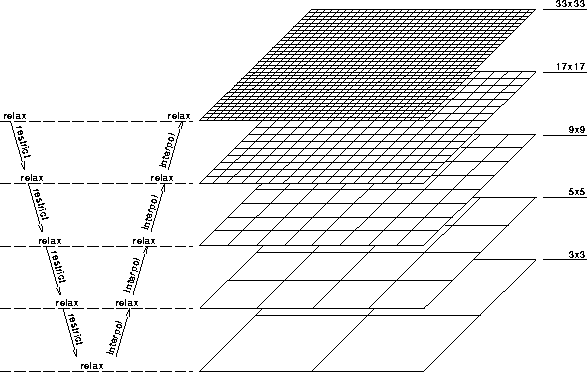
\includegraphics[scale=0.35]{img/02/multigrid.png}
\caption[Multigrille]{Vue des différents niveaux de grilles et du V-cycle.
 Image extraite de \href{http://MGNet.org}{MGNet.org} }
\label{fig:mgrid}
\end{center}
\end{figure}	

%\begin{figure}[htbp]
%\begin{center}
%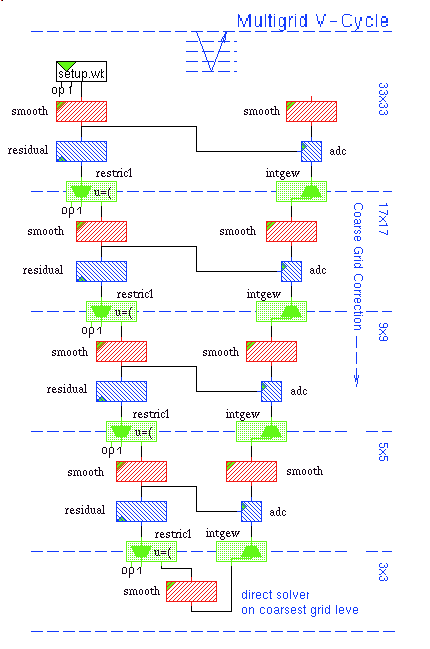
\includegraphics[scale=0.35]{img/02/Vcycle.png}
%\caption{\textbf{Description du V-cycle.} Image extraite de \href{http://MGNet.org}{MGNet.org}}
%\label{Description du V-cycle}
%\end{center}
%\end{figure}		

\subsection{Implémentation dans EMMA}
Dans EMMA, la potentiel est calculé par multigrille sur la grille coarse et utilise l'arbre \ac{AMR} pour gérer les sous-niveaux.
Sur les niveaux raffinés la relaxation est effectuée par Gauss Siedel rouge/noir.
La solution déterminée sur les niveaux grossiers est projetée sur les niveaux raffinés, la solution anticipée est déjà proche de sa vraie valeur. 
Il en résulte une convergence rapide.

Pour des raisons techniques, on prendra garde lors de calcul en parallèle, à utiliser un niveau minimum de telle sorte que chaque processeur dispose au minimum d'un oct lors du calcul sur la grille grossière du multigrille.
Le niveau minimum du V-cycle est : 

\begin{equation}
L_{min} = 1 + ceil \left(\frac{log_2(N_{cpu})}{3}  \right) 
\end{equation}


%\subsection{Liste chaînée de particule}
%\label{sec:chainepart}
%La gestion des particules dans EMMA utilise le principe de la liste chaînée déjà abordée pour les OCT. %TODO ref
%A chaque cellule est associée  un pointeur vers une particule de tète.
%Si ce pointeur est NULL, la cellule ne contient pas de particule.
%Les particules entrant dans cette cellule seront ajoutées a la liste chaînée.
%On prendra garde a gérer cette liste au moment du raffinement et du déraffinement des cellules.
%
%\subsection{Le pas de temps}
%
%Le pas de temps sera calculer de telle sorte a respecter la condition de Courant.
%Une particule ne doit pas se déplacer de plus d'une fraction de case a chaque pas de temps.


%	    dtloc=0.1*SQRT(2.*M_PI/(3.*(curoct->cell[icell].gdata.d+1.)*aexp));
%\begin{equation}
%
%\end{equation}



%%%%%%%%%%%%%%%%%%%%%%%%%%%%%%%%%%%%%%%%%%%%%%%%%%%%%%%%%%%%%%%%%%%%%%%%%%%%%%%%%%%%%%%%%%%%%%%%%%%%%%%%%%%%%%%%%%%%%%%%%%%%%%%%%%%%%%%%%%%%%%%%

\clearpage
\section{Hydrodynamique et la physique baryonique}
\label{sec:hydro}
%solveur hydro
%partie la plus intensive en calcul

Le moteur hydrodynamique est certainement la partie du code la plus complexe et c'est aussi celle sur laquelle j'ai le moins travaillé.
Je vais tout de même en exposer les grandes lignes, mais cette partie sera moins étoffée que celles des autres moteurs physiques.

Comme nous l'avons vu plus tôt (cf \ref{sec:nucleosynthese_primordiale}), l'Univers est constitué d'une grande quantité d'hydrogène et d'hélium sous forme gazeuse.
Dans le cas de l'étude de l'\ac{EoR} la physique du gaz est centrale, car l'objectif est précisément de déterminer les propriétés physicochimiques de ce gaz, et leurs impacts sur la formation des galaxies.
Ici, la physique du gaz est régie par les equations d'Euler auto-gravitantes car le gaz est principalement soumis à deux forces : sa pression interne et la gravité.
Le système d'équations à résoudre est:

\begin{equation}
\begin{cases}

{ \frac{ \partial \rho }{ \partial t } + \nabla \cdot (\rho \vec{v}) = 0}, \\
\\
{ \frac{ \partial }{ \partial t } (\rho \vec{v}) + \nabla \cdot (\rho \vec{v} \otimes v + P1\!\!1 )  = -\rho\nabla \phi }, \\
\\
{ \frac{ \partial E }{ \partial t } + \nabla \cdot [ \rho v (E+p)\vec{v} ] = -\rho \vec{v} \cdot \nabla \phi },

\end{cases}
\end{equation}
\label{eq:hydro}
%+ \rho^2 \Lambda
%$\Lambda$ est la fonction de refroidissement.

avec ;
$\rho = \rho(\vec{x},t)$,
$ \vec{v} = (u,v,w)^T$

Ce système exprime la conservation de la masse, de l'impulsion et de l'énergie et pour être résolu, il nécessite l'introduction d'une equation de fermeture, ou équation d'état.
Nous considérerons ici le cas d'un gaz parfait monoatomique, son équation d'état sera donc:

%\begin{equation}
%P=(\gamma - 1) \rho \epsilon, 
%\end{equation}
%avec l'indice adiabatique $\gamma = 5/3$.
%
%L'énergie totale est donc :
\begin{equation}
E = \frac{\rho}{2	}\vec{v}^2 + \frac{P}{\gamma -1}
\end{equation}
avec l'indice adiabatique $\gamma = 5/3$.


%\begin{equation}
%p=\rho k T, 
%\end{equation}
%avec $k=1.38064852 \cdot 10^{-23} \left[ \mathrm{m^2 \cdot kg \cdot s^{-2} \cdot K^{-1}} \right] $ la constante de Boltzmann.

%\begin{itemize}
%\item PDE
%\item IC
%\item BC
%\end{itemize}


%\begin{equation}
% \frac{\partial U}{\partial t} + \nabla \cdot (F(U)) = S(U), 
%\label{eq:rad_generale}
%\end{equation}
%
%avec $U$ le vecteur des quantité conservées, $F$ la fonction de flux, et $S$ le terme source. Pour la résolution du transport des photons (sans terme source), on retrouve :



En analyse numérique ce système sera réécrit sous la forme:

\begin{equation}
U_t+F_x(U) = S(U),
\label{eq:conservation}
\end{equation}

avec:
\begin{equation}
\begin{array}{c}

U=
\left(
\begin{array}{c}
{ \rho}\\
{\rho u}\\
{\rho v}\\
{\rho w}\\
{\rho E}
\end{array}
\right),
\\
F(U)=
\left(
\begin{array}{ccc}
\rho u & \rho v & \rho w \\ 
\rho u^2 +P & \rho uv & rho uw \\ 
\rho uv & \rho v^2 +P & rho vw \\ 
\rho uw & rho vw &\rho w^2 +P \\ 
(\rho \epsilon + P)u & (\rho \epsilon + P)v & (\rho \epsilon + P)w
\end{array} 
\right)
\\
S(U) =
\left(
\begin{array}{c}
{ 0}\\
{\rho \Phi_x}\\
{\rho \Phi_y}\\
{\rho \Phi_z}\\
{- \rho u \cdot \nabla \Phi + \Lambda }
\end{array}
\right),
\end{array} 
\end{equation}

où $U$ est le vecteur des quantité conservées, $F$ la fonction de flux, et $S$ le terme source.

%,
%F(U)=
%\begin{cases}
%{ \rho u}\\
%{ \rho u^2+p}\\
%{ \rho uv}\\
%{ \rho uw}\\
%{ u(E+p)}
%\end{cases}
\subsection{Le problème de Riemann et volumes finis}

L'idée de base du moteur hydrodynamique est de décomposer le domaine en cellules dans lesquelles les grandeurs seront localement constantes (Piecewise constant approximation).
L'objectif est ensuite de résoudre localement le système d'équations d'Euler à chaque interfaces de cellule pour obtenir l'évolution globale du système.
Chaque interfaces devient donc un problème de Riemann.
Considérant un système, régi par des équations de conservations, aillant comme état initial deux milieux homogènes de densité constante, séparé par une continuité (cf figure \ref{fig:riemann}), qu'elle sera son évolution?

%Nous aurons donc accès aux flux de matière et d'énergie entre les cellules pour pouvoir calculer l'état suivant  
%Connaissant l'état d'un système régit par des équation de conservation hyperbolique de type Euler a un instant donné.
%Le problème de Riemann consiste a considérer l’évolution d'un system d’équations différentielles à partir d'une condition initiale.
%En aillant l’état d'un système régis par des equations différentielles un instant donné, qu'elle sera sont évolution?

\begin{figure}
        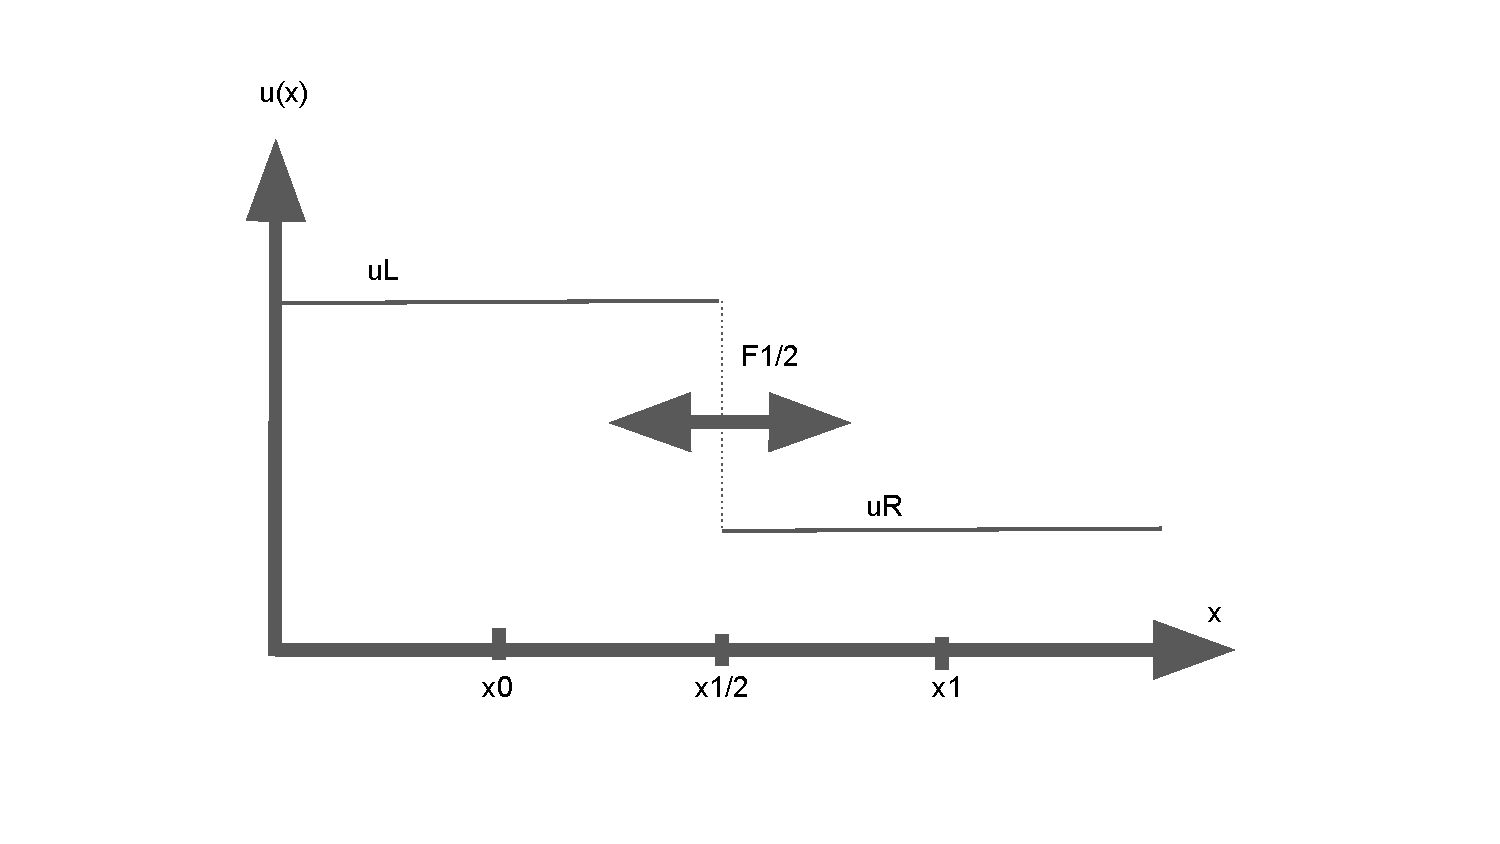
\includegraphics[width=.95\linewidth]{img/02/riemann.pdf} 
        \caption[Problème de Riemann]{Problème de Riemann. Quelle sera l'évolution d'un système hydrodynamique considérant de telles conditions initiales.  
 		\label{fig:riemann}
 		}
\end{figure}

Il existe différents solveur de Riemann.
Contrairement à la résolution de l’équation de Poisson, il n'est plus possible d'utiliser une discrétisation à base de différence finie.

Une différence finie centrée peut être décomposée en deux différence finies : 
\begin{equation}
\frac{d u}{dx} \approx \frac{u_{i+1}  + u_i}{\Delta x} 
\end{equation}

%Dans le premier cas, la discrétisation pourra s'écrire : 
La propagation d'une onde a la vitesse $a$ pourra être discrétisée en utilisant.

\begin{equation}
\frac{u_i^{t+1} + u_i^t }{\Delta t}   +a \frac{u_{i+1}^t  + u_i^t}{\Delta x} = 0
\end{equation}

En fonction du signe de $a$, on parlera de méthode UPWIND ou DOWNWIND.
Il est possible de montrer à l'aide d'une analyse de von-Neumann (cf \cite{toro1999riemann} que la méthode UPWIND est stable sous certaine condition, et que la méthode DOWNWIND est inconditionnelement instable.
Or il n'est pas possible de connaitre à l'avance le signe de $a$, la discrétisation par différence finies ne s'applique donc pas à ce problème. 
Le principe de cette méthode est de ne plus calculer directement l'évolution des grandeurs au sein des cellules mais de passer par l'intermédiaire du calcul des flux entre elles.
On parlera de discrétisation par volumes finis.



%\subsection{Discrétisation du problème.}
%
%Contrairement à la résolution de l’équation de Poisson, il n'est plus possible d'utiliser une discrétisation des dérivées à l'aide d'un différence finie centrée.
%Nous allons rapidement voir pourquoi dans cette section.
%
%Une différence finie centrée peut être décomposée en deux différence finies : 
%\begin{equation}
%\frac{d u}{dx} \approx \frac{u_{i+1}  + u_i}{\Delta x} 
%\end{equation}
%
%\begin{equation}
%\frac{d u}{dx} \approx \frac{u_i  + u_{i+1}}{\Delta x} 
%\end{equation}
%
%Considérons que nous voulons résoudre l'équation :
%\begin{equation}
%\frac{du}{dt} + a\frac{du}{dx} = 0
%\end{equation}
%
%Dans le premier cas, la discrétisation pourra s'écrire : 
%%la propagation d'une onde a la vitesse $a$ pourra être discrétisée en utilisant.
%
%\begin{equation}
%\frac{u_i^{t+1} + u_i^t }{\Delta t}   +a \frac{u_{i+1}^t  + u_i^t}{\Delta x} = 0
%\end{equation}
%
%\begin{equation}
%u_i^{t+1}  = u_i^t +  c \left( u_{i+1}^t  + u_i^t \right) 
%\end{equation}
%
%ou : 
%
%\begin{equation}
%c= \frac{a \Delta t}{\Delta x},
%\end{equation}
%est le nombre de Courant
%
%A l'aide d'une analyse de von-Neumann (cf \cite{toro1999riemann}), on montre que la stabilité de ce schéma dépend du signe de a, la vitesse de propagation de l'onde.
%
%\begin{itemize}
%\item si a est positif, ce schéma est conditionnellement stable (la condition étant que la condition de Courant soient respectée : $0<c<1$) .
%Ce schema est appélé méthode UPWIND.
%
%\item A l'inverse on montre que que dans le cas de la seconde différence finie, le schéma est inconditionnellement instable. 
%Ce shema est appelée méthode DOWNWIND.
%\end{itemize}
%
%Seule la méthode upwind permet de suivre correctement la propagation d'onde.
%Le problème est qu'a trois dimension, il est impossible de respecter cette condition pour un système quelconque.
%% déterminer dans quelle direction se propage une onde quelconques.
%
%De plus il a été montré que cette méthode n'est pas conservative, et qu'elle était incapable de suivre les chocs (fortes discontinuités)
%


%\subsection{Méthode de Godunov}
%
%
%introduction aux volumes finis
%consiste a estimer le flux aux interfaces des cellules.
%

%\subsection{discretisation}
Godunov \cite{MR0119433} a été le premier à introduire une méthode pour la résolution exacte de ce système.
%répondu à ce problème et introduit une méthode conservative.
Son approche consistait à discrétiser l'équation \ref{eq:conservation} de la manière suivante : 

\begin{equation}
\frac{ u^{t+1}_i - u^t_i }{\Delta t} + \frac{ F^t_{i+1/2} - F^t_{i-1/2} }{\Delta x} =0,
\label{eq:rad_solver}
\end{equation}

ou $F^t_{i+1/2}$ et $F^t_{i-1/2}$ sont les flux numérique intercellules, ou flux de Godunov, une estimations des flux physique.
Tout le problème réside dans le calcul de ces flux aux interfaces. % : $F^t_{i+1/2}$
Différentes méthodes ont été développées, et celle retenue dans EMMA est la méthode HLL/HLLC.
%\subsection{Méhtode HLL et HLLC }
La méthode de HLL Harten, Lax et van Leer  est une méthode pour résoudre approximer les flux de Godunov dans le cas de la résolution en 3D des équation d'Euler.
La méthode HLL a été modifié par Toro 1992 et a donné lieu à la méthode HLLC, plus robuste.

%recalculation des flux entre les cellules

%\subsection{MUSCL et Minmod}
Si dans le problème de Riemann, les deux parties sont considérées avoir des densités constantes, il est possible de considérer des schémas d'ordres supérieurs.
Par exemple le schéma \ac{MUSCL} introduit par \cite{1979JCoPh..32..101V},  consiste à considérer une valeur dans la cellule, non plus constante mais interpolée linéairement (cf figure\ref{fig:MUSCL}).

\begin{figure}
        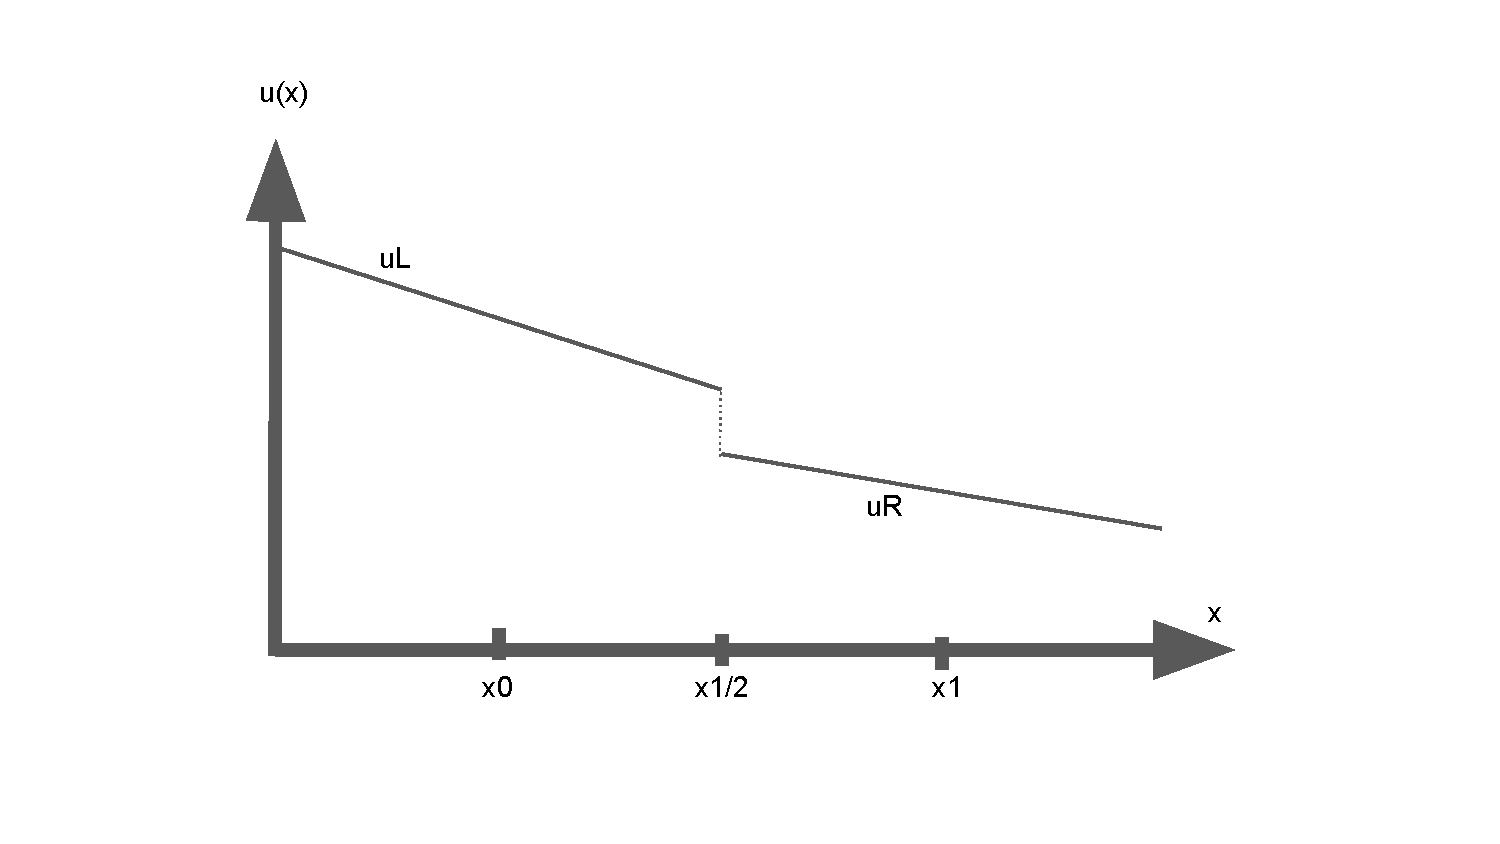
\includegraphics[width=.95\linewidth]{img/02/MUSCL_minmod.pdf} 
        \caption[Méthode MUSCL]{Avec le \ac{MUSCL} la densité au sein des cellules est interpolée linéairement, ce qui améliore le calcul du flux aux interfaces.
        La pente est cependant limitée par la méthode du Minmod.
 		\label{fig:MUSCL}
 		}
\end{figure}



\subsection{Le pas de temps}

Le pas de temps respecte encore une fois la condition de courant qui s'exprime ici sous la forme.:

\begin{equation}
\frac{dx * CFL }{3*(max(v) + c_s)}
\end{equation}

avec $c_s = \sqrt{\gamma P/\rho}$ dans le cas d'un gaz parfais.

%%%%%%%%%%%%%%%%%%%%%%%%%%%%%%%%%%%%%%%%%%%%%%%%%%%%%%%%%%%%%%%%%%%%%%%%%%%%%%%%%%%%%%%%%%%%%%%%%%%%%%%%%%%%%%%%%%%%%%%%%%%%%%%%%%%%%%%%%%%%%%%%

\clearpage
\section{Radiation et énergie ionisante}
\label{sec:rad_solver}


L'objectif de cette section est de présenter les bases de la physique radiative, du transfert du rayonnement (RT) à son interaction avec les baryons.
Ce moteur se déroule en deux temps.
Premièrement, il faut calculer la propagation du rayonnement, on appelles cette étape \textit{le transport} des photons.
Deuxièmement, il faut le couplage entre le rayonnement et le gaz, c'est a dire calculer l'impact \textit{chimie} du gaz.
Nous nous intéresserons ici uniquement au transfert d'énergie ionisante.
Nous verrons dans un premier temps le système d'équation a résoudre, puis dans un second temps, les méthodes de discrétisation.

\subsection{L'équation du transfert du rayonnement}

L'équation du transfert du rayonnement lie l'évolution de l'intensité spécifique $I_\nu(\vec{x},\vec{n},t)$, au champ de sources $\eta_\nu(\vec{x},\vec{n},t)$, en fonction du coefficient d'absorption $\kappa_\nu(\vec{x},\vec{n},t)$ :
\begin{equation}
\frac{1}{c} \frac{\partial I_\nu}{\partial t} + \vec{n}\cdot \vec{\nabla} I_\nu = \eta_\nu - \kappa_\nu I_\nu 
\label{eq:rad}
\end{equation}

Le coefficient d'absorption s'exprime en fonction de la section efficace de photo-ionisation de l'hydrogène neutre $\sigma_\nu$ et de la densité d'hydrogène neutre $n_H$ :
\begin{equation}
\kappa_\nu(\vec{x},\vec{n},t) = \sigma_\nu n_H.
\end{equation}

Il existe deux grandes famille de code de transfert de rayonnement.
\begin{itemize}
\item La première famille utilise une représentation très physique de la lumière, et simule la radiation à l'aide de rayons se propageant dans l'espace.
ce spnt des méthodes dite de lancer de rayons.
Dans le cas ou la vitesse de ces rayon est infinie, on appelle ces méthodes de Monté Carlo.
CRASH \citep{2003MNRAS.345..379M}, C$^2$RAY\citep{2006NewA...11..374M}.
Ce type de code utilise une principe qui se rapproche physiquement de la vraie nature de la lumière.
Chaque source lance un certain nombre de groupe de photon, qui vont se propager et interagir avec le milieu.
Plus les sources sont nombreuses, plus le nombre de groupe de photons à suivre devient important, et plus le cout numérique l'est également.

\item La seconde, celle utilisée dans EMMA, repose sur le principe de considérer la lumière comme un fluide. \citep{gnedin_multi-dimensional_2001, aubert_radiative_2008}.
Ces méthodes dites méthodes aux moments utiliseront donc les même concepts que le moteur hydrodynamique, mais avec un système initial d'équations différentes. 
EMMA utilise une approximation du moment au premier ordre, son moteur repose sur l'\textit{approximation M1} \citep{levermore_relating_1984}.
Son principal avantage est que le coût numérique est indépendant du nombre de sources.
\end{itemize}


\subsection{Méthode des moments}
Les deux premiers moments (d'ordre 0 et 1) de l'équation \ref{eq:rad} s'exprime sous la forme:
\begin{equation}
\begin{cases}
\frac{ \partial N_\nu }{ \partial t } + \vec{\nabla} \cdot \vec{F}_\nu = -\kappa_\nu c  N_\nu + S_\nu,\\
\frac{ \partial \vec{F} }{ \partial t } + c^2 \vec{\nabla} P_\nu = -\kappa_\nu c \vec{F}_\nu ,
\end{cases}
\label{eq:densite_energie}
\end{equation}
avec:
$\vec{F}_\nu$ le flux radiatif, 
$P_\nu $ la pression radiative (sous forme tensorielle),
et $S_\nu = \dot{N}_\nu^* + \dot{N}_\nu^{rec}$ le taux d’émission de photon due aux sources $\dot{N}_\nu^*$ et à la recombinaison $ \dot{N}_\nu^{rec}$.

\subsection{Relation de fermeture et approximation M1}

De la même manière que l'équation d'état des gaz parfait est utilisée pour fermer le système d'équations d'Euler (voir \ref{sec:hydro}).
Dans le cas du transfert du rayonnement, la fermeture du système se fait par l'intermédiaire de l’équation d’état :

\begin{equation}
 P_\nu = D N\nu ,
\label{eq:fermeture}
\end{equation}

ou $D$ est le tenseur d’Eddington et est approximé par le modèle M1 \citep{levermore_relating_1984}%,gonzalez2005} :

\begin{equation}
\begin{cases}

D = \frac{ 3\chi -1 }{2} \mathbb{1} + \frac{ 1 - \chi }{2} \vec{n} \otimes \vec{n} , \\
\\
\chi(\vec{f}_\nu) = \frac{ 3+4 |\vec{f}_\nu|^2 }{5+2\sqrt{4-3|\vec{f}_\nu|^2}} , \\
\\
\vec{f}_\nu = \frac{ \vec{F}_\nu }{c N\nu }  ,

\end{cases}
\label{eq:tenseur}
\end{equation}


\subsection{Vitesse de la lumière réduite}
\label{sec:RSLA}

La lumière étant extrêmement rapide, le suivi de son évolution demande un pas de temps réduit du fait de la condition de Courant : $ c \leq \Delta x / \Delta t $.
D'une manière générale, le pas de temps radiatif est plusieurs ordres de grandeur plus petit que celui de l'hydrodynamique.
Or, les simulation cosmologique utilise l'approximation Newtonienne: les processus entrant en jeux ont des vitesses très inférieures à celle de la lumière.
L'idée est de diminuer la vitesse de la lumière dans le code tout en restant dans le domaine de l'approximation newtonienne.
Cette approximation s'appelle approximation de la vitesse de la lumière réduite ou \ac{RSLA}.
On introduite $c_{num}$ la vitesse de la lumière numérique réduite en fonction de $c$ la vitesse de la lumière physique.
\begin{equation}
c_{num} = \tilde{c} \cdot{c},
\end{equation}
avec $\tilde{c}$ le facteur de proportionnalité. 
Par exemple utiliser $\tilde{c}=0.1$ permet de réaliser 10 fois moins de pas de temps, et donc 10 fois moins de calcul.
J'ai mené une étude dans le but de quantifier l'influence de la vitesse de la lumière réduite sur la propagation des fronts d'ionisation.
Cette étude sera présenté en détails dans la section \ref{sec:lightspeed}.

\subsection{Groupes de photons}
\label{sec:groupedephotons}

Il n'est pas possible avec la méthode au moment de considérer directement un spectre d'émission.
Le spectre doit être discrétisé, c'est a dire qu'il devra être découpé en un certain nombre de groupe, et chaque groupe disposera des caractéristique moyenne de sa portion du spectre.
Le problème est que chaque groupe de photon devient un fluide a simuler a part entière et le coût numérique augmente rapidement avec le nombre de groupes. 
%Il est possible de choisir un nombre arbitraire de groupes, mais il faut prendre en compte que chaque groupe devient l'équivalent d'un fluide dont on veut suivre l'évolution.
%l'augmentation du nombre de groupe devient vite coûteux en terme de temps de calculs.
%Ce profil d’émission ionisante peut être découper en différents "groupe de photons" (cf section \ref{sec:groupedephotons}).

Prenons l'exemple d'un spectre d'émission arbitraire.
L’énergie moyenne d'un photon dans un groupe d'énergie comprissent entre $\nu_1$ et $\nu_2$ est calculée de la manière suivante:
\begin{equation}
<E> = \frac{1}{N} \int_{\nu_1}^{\nu_2} N_\nu h \nu d\nu
\end{equation}
et la section efficace d'interaction:
\begin{equation}
\sigma_E = \frac{1}{N<E>} \int_{\nu_1}^{\nu_2} N_\nu h \nu d\nu
\end{equation}

On prendra généralement la première borne au niveau de l'énergie d'ionisation de l'hydrogène : $\nu_1=13.6eV$.
Dans le cas où on ne considère qu'un seul groupe, les intégrations sont réalisées jusqu'à l'infini : $\nu_2= + \inf$.
J'ai également pu tester le cas de trois groupes, dans ce cas les bornes sont arbitrairement prisent aux niveaux des énergie d'ionisation de l'hélium : 
$\nu_2= 24.6 eV$, $\nu_3= 54.4 eV $, $\nu_4= + \inf$.

J'ai implémenté la possibilité de découper les groupes, non seulement en énergies, mais aussi en temps, car il est possible de considérer une évolution temporelle du spectre d'émission.
Dans ce cas l'énergie moyenne d'un groupe devient : 
\begin{equation}
<E> = \frac{1}{N}  \int_{t_1}^{t_2}  \int_{\nu_1}^{\nu_2} N_{(\nu,t)} h \nu d\nu dt
\end{equation}
Une opération identique est réalisée pour la section efficace.

Après de rapides tests, le ratio cout de calcul sur amélioration des prédictions n'est pas en faveur de l'augmentation du nombre de groupes, du moins dans le cas des résolutions considérées pendant ma thèse.
En pratique je n'ai travaillé qu'avec un seul groupe de photons.

\subsection{La chimie}
\label{sec:chimie}

La chimie fait le lien entre le moteur radiatif et le moteur hydrodynamique.
C'est à ce moment qu'est appliquée l'énergie apportée par la radiation au gaz et que le gaz va être chauffé par la radiation.
A l'inverse, et contrairement au transport , la chimie est non conservative, et c'est a se moment que la gestion du refroidissement du gaz à lieu.
En effet, une partie des photon ionisant vont être intercepté par le gaz et réémis dans une autre partie du spectre.
Cette réémission est numériquement interprété comme une perte d'énergie.

Le système d'équations à résoudre lie la densité de photons, le flux de photons, l'état d'ionisation et l'énergie interne : 

\begin{equation}
\frac{dN}{dt} = S - c \sigma_N n_H N + \left( \alpha_A(T)  - \alpha_B(T) \right) x^2n_0^2
\end{equation}
\begin{equation}
\frac{dF}{dt} = - c \sigma_N n_H F
\end{equation}
\begin{equation}
\frac{dn_H}{dt} =  \left( \alpha_A(T)x^2  - \alpha_B(T)x (1-x) \right) n_0^2 - c \sigma_N n_HN
\end{equation}
\begin{equation}
\frac{de}{dt} = c n_H \Sigma_E N - \Lambda_{(n_0,x,T)}
\end{equation}

où $n_H$ est la densité d'atomes d'hydrogène (en nombre).
Les taux de réaction chimique $\alpha_A(T)$, $\alpha_B(T)$ et $\beta_(T)$ sont repris de tables de \cite{theuns_p^3m-sph_1998} et les sections efficace d'interactions de \cite{hui_equation_1997}.

Il est possible de considérer que toute l'énergie de recombinaison est localement réabsorbée en forçant $\alpha_A(T) = \alpha_B(T)$.
Ceci est connu sous le nom de \ac{OTSA}.

Les processus chimique agissant sur des échelles de temps courtes par rapport au transport des photons, le pas de temps sera plusieurs ordres de grandeurs plus faible.
En pratique, a chaque pas de temps radiatif, on effectuera un sous-cyclage sur le pas de temps chimique.
Après chaque pas de temps chimique, la variation d’énergie est calculée. 
Si celle ci est supérieure a 10\%, le pas de temps est divisée par 2 et l'étape courante est recalculée. (cf \cite{rosdahl_ramsesrt_2013}) 

Étant donné que le processus chimique sont uniquement local (ie ils ne dépendent pas de l'état des cellules voisines) et que la quantité de calcul est relativement importante, le portage du moteur chimique sur \ac{GPU} est très intéressant du point de vue accélération.

\subsection{Transport sur grille de base}
\label{sec:crta}

Le transport sur grille de base ou \ac{CRTA} est une technique visant à restreindre la résolution du champ de radiation dans le but d'en accélérer le calcul.
Dans le cas d'un couplage total entre les différents moteurs physiques, tous les moteur évoluent au rythme le plus contraignant.
%il faut définir le plus petit pas de temps et faire évoluer 
Ce qui fait que, pour chaque pas de temps radiatif, il faut réaliser un pas de temps avec les autres moteurs physique (cf panneau supérieur de la figure \ref{fig:CRTA}).
Dans notre cas, la radiation est plusieurs ordres de grandeurs plus contraignante que l'hydrodynamique ou la gravitation.
Donc le nombre de pas de temps hydrodynamique et gravitationnel nécessaire sont largement surestimés, et le coût numérique explose.

Dans le cas de la \ac{CRTA}, le transport des photons n'est réalisé que sur la grille de base, et non sur les niveaux raffinées (cf panneau inférieur de la figure \ref{fig:CRTA}).
Ce qui a pour effet d'augmenter artificiellement la taille du pas de temps radiatif, du fait de la condition de Courant.
La densité de photon calculée sur la grille de base est ensuite projeté sur les niveaux raffinés, ces derniers ressentant l'équivalent d'un "fond UV" local.

Actuellement, la \ac{CRTA} n'est possible que sur le niveau de base.
Un amélioration possible serait de pouvoir définir le niveaux de projection de la radiation pour pouvoir, en fonction des besoins, faire varier le poids de la radiation dans le calcul.


\begin{figure}
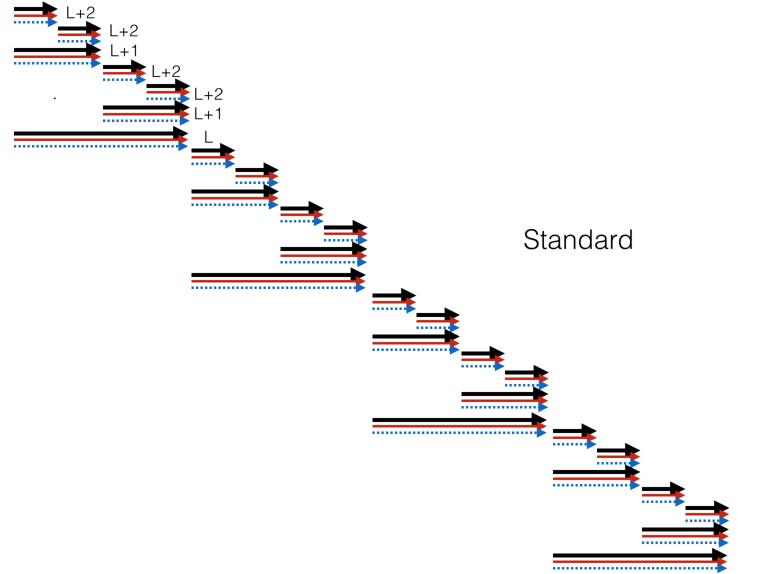
\includegraphics[width=.95\linewidth]{img/02/revz_crad_std.png}
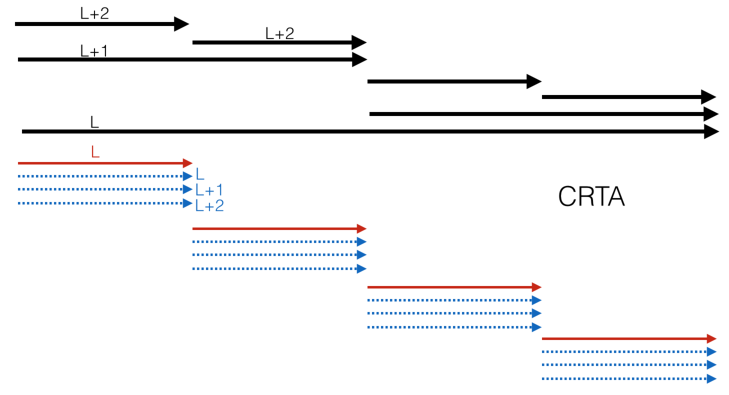
\includegraphics[width=.95\linewidth]{img/02/revz_crad.png}
\caption[CRTA]{Gestion de l'évolution de la radiation dans le cas de la \ac{CRTA}.
En noir les moteurs dynamiques, en rouge le transport des photons, en bleu la chimie.
Le transport des photons n'est réalisé que sur la grille de niveau de base.
Le nombre d'appels aux moteurs hydrodynamique et gravitationnel est significativement réduit. 
\label{fig:CRTA}}
\end{figure}
